% P4 processing block diagram, grounded in the implementation call paths.
% Compile from this directory with:
%   latexmk -pdf -interaction=nonstopmode p4_algorithm_processing.tex
\documentclass[tikz,border=8pt]{standalone}

\usepackage[T1]{fontenc}
\usepackage{lmodern}
\usetikzlibrary{arrows.meta,fit,positioning,shapes.geometric}

\definecolor{p4app}{HTML}{DCEBFA}
\definecolor{p4setup}{HTML}{FFF1C9}
\definecolor{p4core}{HTML}{DDF2DF}
\definecolor{p4optional}{HTML}{EADFF4}
\definecolor{p4output}{HTML}{E8E8E8}
\definecolor{p4line}{HTML}{34495E}

\tikzset{
  >={Latex[length=2.4mm]},
  flow/.style={-Latex, draw=p4line, line width=0.65pt},
  feedback/.style={flow, dashed},
  block/.style={
    rectangle,
    rounded corners=1.5pt,
    draw=p4line,
    line width=0.55pt,
    align=center,
    inner xsep=5pt,
    inner ysep=4pt,
    font=\sffamily\footnotesize,
    minimum height=10mm
  },
  app/.style={block, fill=p4app},
  setup/.style={block, fill=p4setup},
  core/.style={block, fill=p4core},
  optional/.style={block, fill=p4optional},
  output/.style={block, fill=p4output},
  decision/.style={
    diamond,
    aspect=2.0,
    draw=p4line,
    fill=white,
    line width=0.55pt,
    align=center,
    inner sep=1.5pt,
    font=\sffamily\scriptsize
  },
  group/.style={
    rectangle,
    rounded corners=3pt,
    draw=p4line,
    dashed,
    inner sep=5pt
  },
  edge label/.style={
    fill=white,
    inner sep=1.5pt,
    font=\sffamily\scriptsize,
    text=p4line
  },
  note/.style={font=\sffamily\scriptsize, align=left, text=p4line}
}

\begin{document}
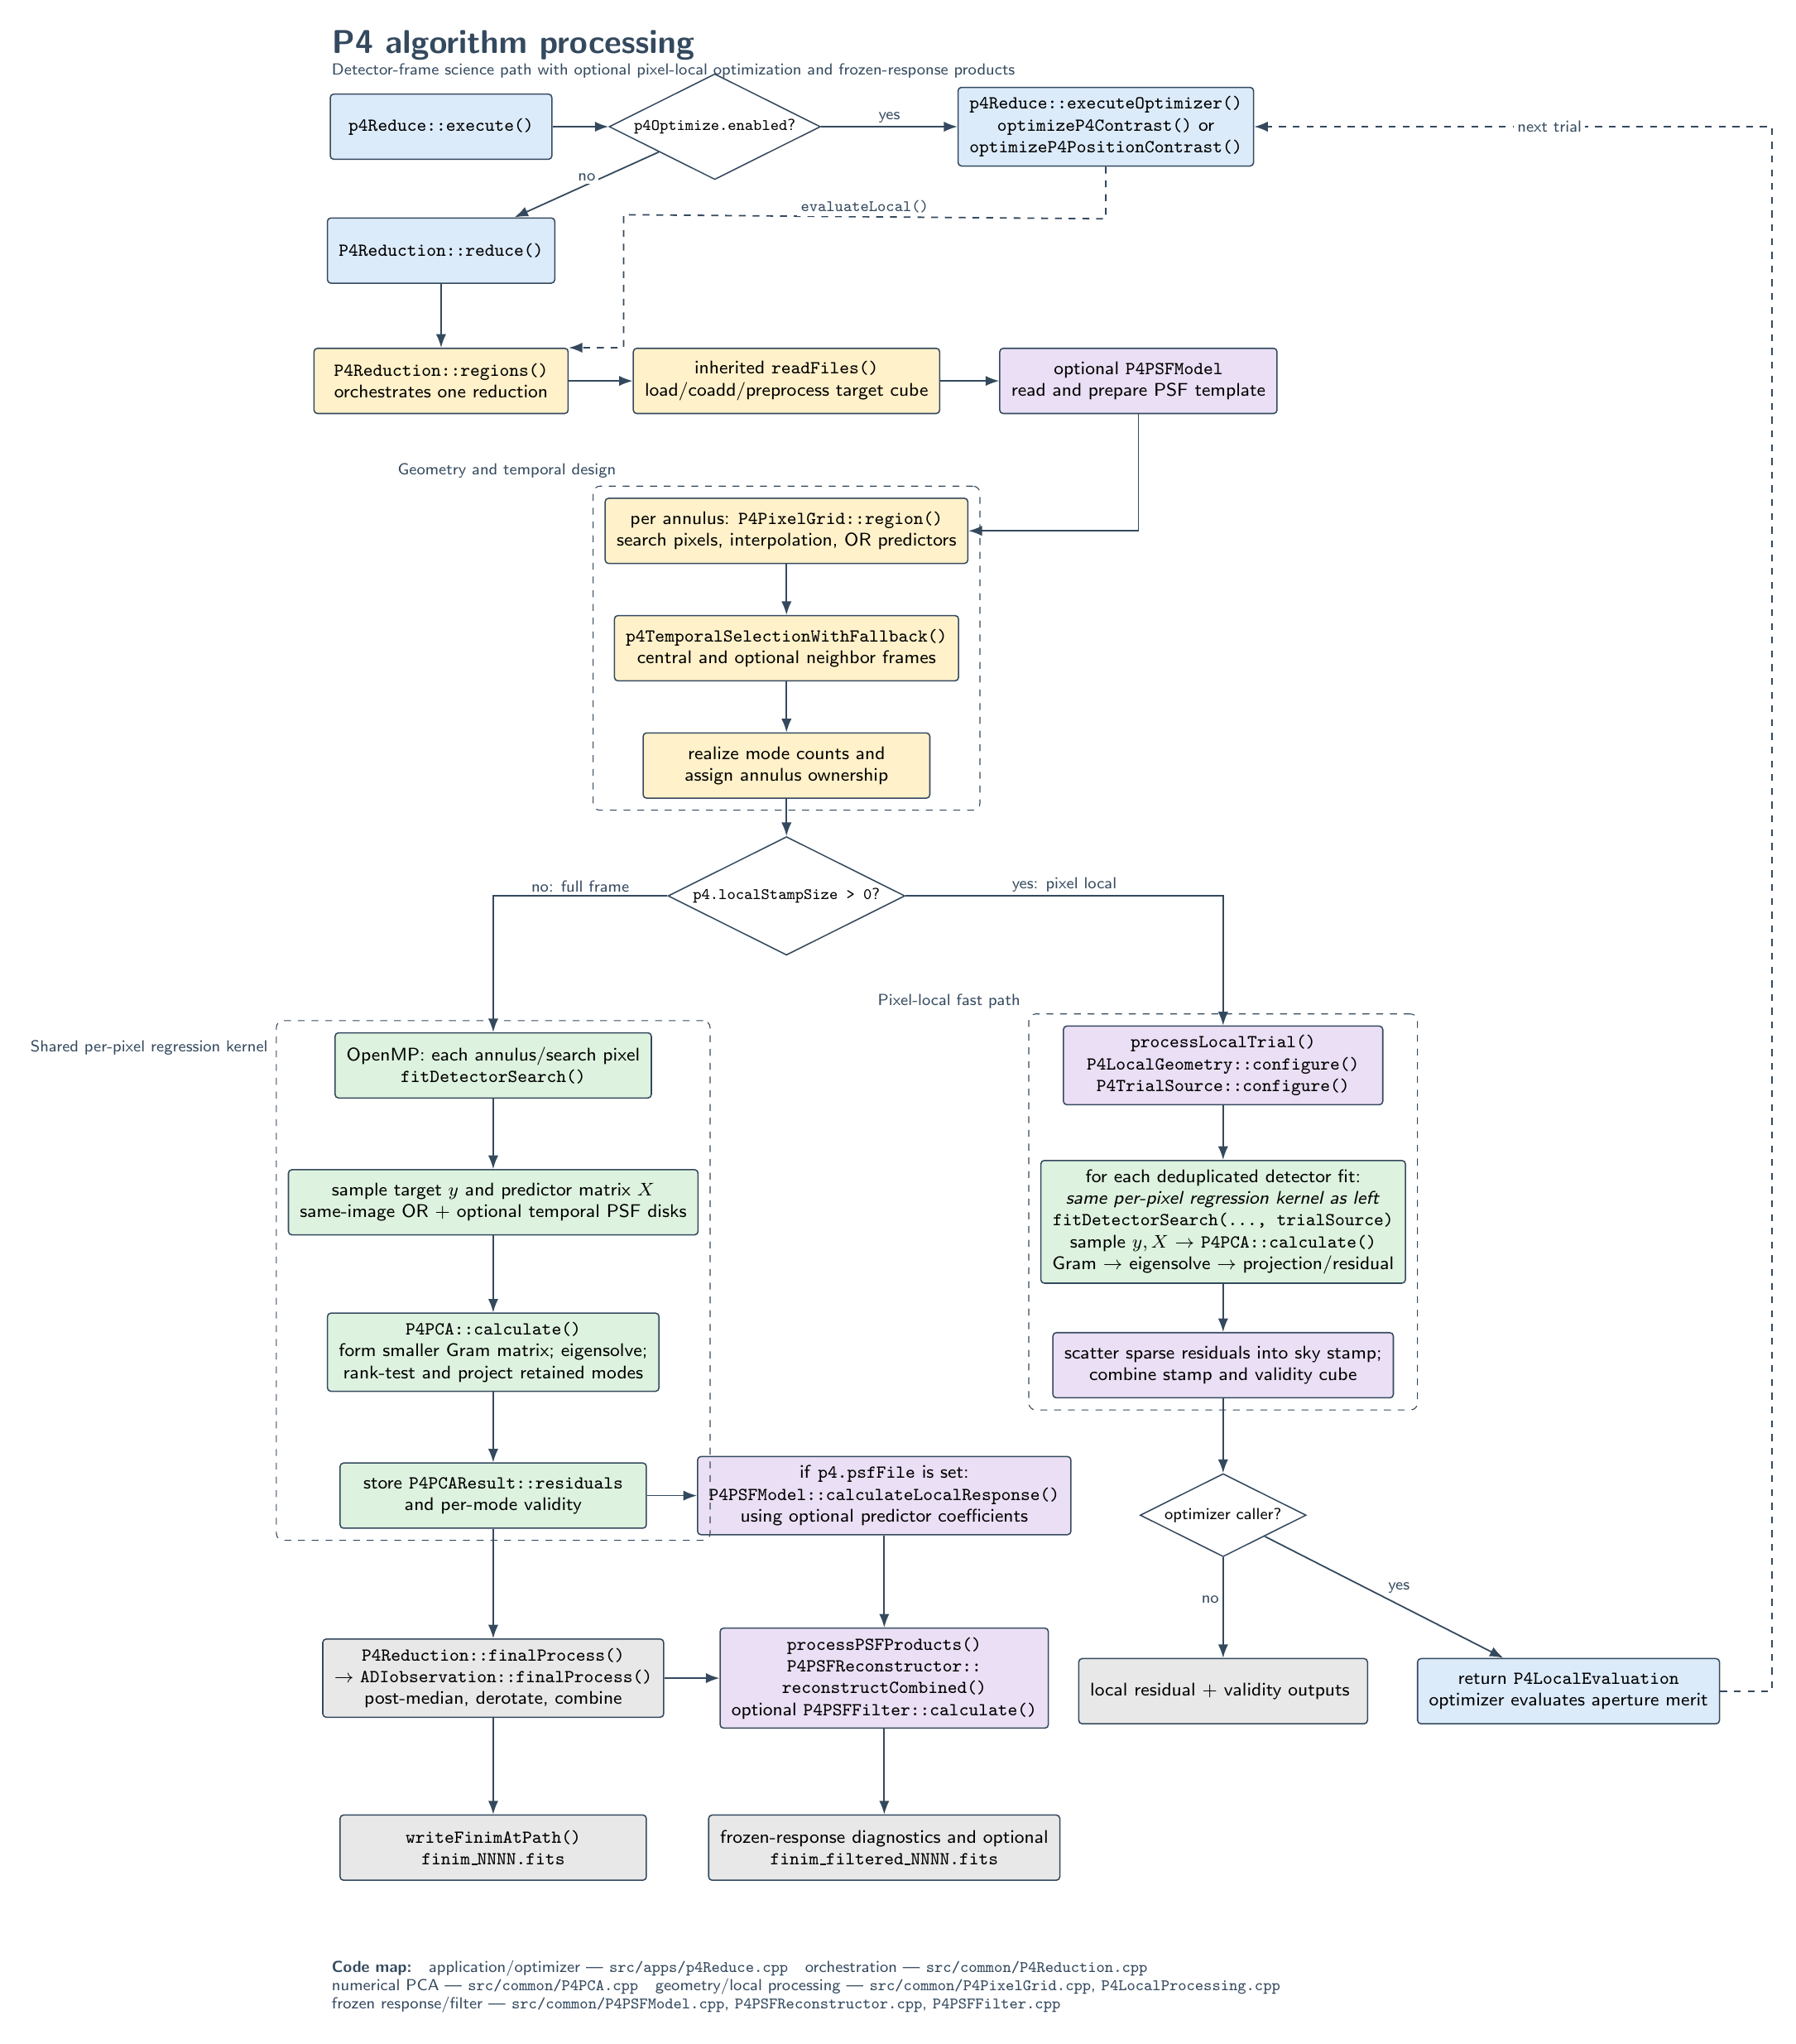
\begin{tikzpicture}
  \node[anchor=west, font=\sffamily\Large\bfseries, text=p4line] at (-9.8,1.25)
    {P4 algorithm processing};
  \node[anchor=west, font=\sffamily\scriptsize, text=p4line] at (-9.8,0.85)
    {Detector-frame science path with optional pixel-local optimization and frozen-response products};

  % Application dispatch.
  \node[app, minimum width=34mm] (execute) at (-8,0) {\texttt{p4Reduce::execute()}};
  \node[decision] (optimizer-enabled) at (-3.8,0) {\texttt{p4Optimize.enabled}?};
  \node[app, minimum width=45mm] (optimizer) at (2.2,0) {
    \texttt{p4Reduce::executeOptimizer()}\\
    \texttt{optimizeP4Contrast()} or\\
    \texttt{optimizeP4PositionContrast()}
  };

  \node[app, minimum width=34mm] (reduce) at (-8,-1.9) {\texttt{P4Reduction::reduce()}};
  \node[setup, minimum width=39mm] (regions) at (-8,-3.9) {
    \texttt{P4Reduction::regions()}\\
    orchestrates one reduction
  };
  \node[setup, minimum width=42mm] (load) at (-2.7,-3.9) {
    inherited \texttt{readFiles()}\\
    load/coadd/preprocess target cube
  };
  \node[optional, minimum width=40mm] (psf-init) at (2.7,-3.9) {
    optional \texttt{P4PSFModel}\\
    read and prepare PSF template
  };

  \draw[flow] (execute) -- (optimizer-enabled);
  \draw[flow] (optimizer-enabled) -- node[edge label, above] {no} (reduce);
  \draw[flow] (optimizer-enabled) -- node[edge label, above] {yes} (optimizer);
  \draw[flow] (reduce) -- (regions);
  \draw[flow] (regions) -- (load);
  \draw[flow] (load) -- (psf-init);

  % Geometry and temporal design.
  \node[setup, minimum width=44mm] (grid) at (-2.7,-6.2) {
    per annulus: \texttt{P4PixelGrid::region()}\\
    search pixels, interpolation, OR predictors
  };
  \node[setup, minimum width=44mm] (temporal) at (-2.7,-8.0) {
    \texttt{p4TemporalSelectionWithFallback()}\\
    central and optional neighbor frames
  };
  \node[setup, minimum width=44mm] (modes) at (-2.7,-9.8) {
    realize mode counts and\\
    assign annulus ownership
  };
  \node[decision] (local-enabled) at (-2.7,-11.8) {\texttt{p4.localStampSize > 0}?};

  \draw[flow] (psf-init.south) |- (grid.east);
  \draw[flow] (grid) -- (temporal);
  \draw[flow] (temporal) -- (modes);
  \draw[flow] (modes) -- (local-enabled);

  % Full-frame regression path.
  \node[core, minimum width=47mm] (fit) at (-7.2,-14.4) {
    OpenMP: each annulus/search pixel\\
    \texttt{fitDetectorSearch()}
  };
  \node[core, minimum width=47mm] (sample) at (-7.2,-16.5) {
    sample target \(y\) and predictor matrix \(X\)\\
    same-image OR + optional temporal PSF disks
  };
  \node[core, minimum width=47mm] (pca) at (-7.2,-18.8) {
    \texttt{P4PCA::calculate()}\\
    form smaller Gram matrix; eigensolve;\\
    rank-test and project retained modes
  };
  \node[core, minimum width=47mm] (residual) at (-7.2,-21.0) {
    store \texttt{P4PCAResult::residuals}\\
    and per-mode validity
  };
  \node[optional, minimum width=47mm] (local-psf) at (-1.2,-21.0) {
    if \texttt{p4.psfFile} is set:\\
    \texttt{P4PSFModel::calculateLocalResponse()}\\
    using optional predictor coefficients
  };
  \node[output, minimum width=47mm] (final-process) at (-7.2,-23.8) {
    \texttt{P4Reduction::finalProcess()}\\
    \(\rightarrow\) \texttt{ADIobservation::finalProcess()}\\
    post-median, derotate, combine
  };
  \node[output, minimum width=47mm] (science-output) at (-7.2,-26.4) {
    \texttt{writeFinimAtPath()}\\
    \texttt{finim\_NNNN.fits}
  };
  \node[optional, minimum width=49mm] (psf-products) at (-1.2,-23.8) {
    \texttt{processPSFProducts()}\\
    \texttt{P4PSFReconstructor::}\\
    \texttt{reconstructCombined()}\\
    optional \texttt{P4PSFFilter::calculate()}
  };
  \node[output, minimum width=49mm] (psf-output) at (-1.2,-26.4) {
    frozen-response diagnostics and optional\\
    \texttt{finim\_filtered\_NNNN.fits}
  };

  \draw[flow] (local-enabled) -| node[edge label, near start, above] {no: full frame} (fit);
  \draw[flow] (fit) -- (sample);
  \draw[flow] (sample) -- (pca);
  \draw[flow] (pca) -- (residual);
  \draw[flow] (residual) -- (final-process);
  \draw[flow] (residual) -- (local-psf);
  \draw[flow] (local-psf.south) -- (psf-products.north);
  \draw[flow] (final-process) -- (science-output);
  \draw[flow] (final-process) -- (psf-products);
  \draw[flow] (psf-products) -- (psf-output);

  % Pixel-local path and optimizer feedback.
  \node[optional, minimum width=49mm] (local-geometry) at (4.0,-14.4) {
    \texttt{processLocalTrial()}\\
    \texttt{P4LocalGeometry::configure()}\\
    \texttt{P4TrialSource::configure()}
  };
  \node[core, minimum width=55mm] (local-fits) at (4.0,-16.8) {
    for each deduplicated detector fit:\\
    \textit{same per-pixel regression kernel as left}\\
    \texttt{fitDetectorSearch(..., trialSource)}\\
    sample \(y,X\) \(\rightarrow\) \texttt{P4PCA::calculate()}\\
    Gram \(\rightarrow\) eigensolve \(\rightarrow\) projection/residual
  };
  \node[optional, minimum width=49mm] (local-stamp) at (4.0,-19.0) {
    scatter sparse residuals into sky stamp;\\
    combine stamp and validity cube
  };
  \node[decision] (optimizer-return) at (4.0,-21.3) {optimizer caller?};
  \node[output, minimum width=42mm] (local-output) at (4.0,-24.0) {
    local residual + validity outputs
  };
  \node[app, minimum width=45mm] (merit) at (9.3,-24.0) {
    return \texttt{P4LocalEvaluation}\\
    optimizer evaluates aperture merit
  };

  \draw[flow] (local-enabled) -| node[edge label, near start, above] {yes: pixel local} (local-geometry);
  \draw[flow] (local-geometry) -- (local-fits);
  \draw[flow] (local-fits) -- (local-stamp);
  \draw[flow] (local-stamp) -- (optimizer-return);
  \draw[flow] (optimizer-return) -- node[edge label, above left] {no} (local-output);
  \draw[flow] (optimizer-return) -- node[edge label, above right] {yes} (merit);
  \draw[feedback] (merit.east) -- ++(8mm,0) |- node[edge label, near end, right] {next trial} (optimizer.east);
  \draw[feedback] (optimizer.south) -- ++(0,-8mm) -- node[edge label, above] {\texttt{evaluateLocal()}}
    (-5.2,-1.35) |- (regions.north east);

  % Visual grouping and implementation pointers.
  \node[group, fit=(temporal) (grid) (modes), label={[note]above left:Geometry and temporal design}] {};
  \node[group, fit=(fit) (sample) (pca) (residual), label={[note]above left:Shared per-pixel regression kernel}] {};
  \node[group, fit=(local-geometry) (local-fits) (local-stamp), label={[note]above left:Pixel-local fast path}] {};

  \node[note, anchor=north west] at (-9.8,-28.0) {
    \textbf{Code map:}\quad
    application/optimizer --- \texttt{src/apps/p4Reduce.cpp}\quad
    orchestration --- \texttt{src/common/P4Reduction.cpp}\\
    numerical PCA --- \texttt{src/common/P4PCA.cpp}\quad
    geometry/local processing --- \texttt{src/common/P4PixelGrid.cpp}, \texttt{P4LocalProcessing.cpp}\\
    frozen response/filter --- \texttt{src/common/P4PSFModel.cpp}, \texttt{P4PSFReconstructor.cpp},
    \texttt{P4PSFFilter.cpp}
  };
\end{tikzpicture}
\end{document}
